\documentclass[hyper,comprehensive]{MUthesis}
%% options:
%%  doublespace  -- the default, indicates double spacing as per MU
%%                  requirements; use for all final copies
%%  singlespace  -- for early work; not acceptable for final draft
%%  dissertation -- default; indicates this is a dissertation
%%  thesis       -- indicates this is a Master's thesis; changes the default
%%                  for \degree{}{} to Master of Science / M.S.
%%  nolisthyphen -- disallows hyphenation in the Table of Contents and
%%                      the list of figures/tables; only use if the graduate
%%                      school or your committee complain
%%  nohyphen     -- disallows hyphenation /everywhere/; don't use unless
%%                  someone complains (and even then, fight back!)
%%  hyperpages   -- default; loads hyperref with stripped down options
%%  hyper        -- loads hyperref with page labels and invisible links
%%  nohyper      -- turns off loading of hyperref, which is used only to
%%                  fix page labels (so that i is called i, not 1, in the PDF);
%%                  use this if you want to load hyperref with other options
%%
%%  All other options are passed as-is to the "report" class; the default size
%%  is 12pt, but you can specify 10 or 11 pt (or any other size supported by
%%  "report")

\usepackage{amsmath}
\usepackage{physics}
\usepackage{txfonts}
\usepackage{graphicx}
%\usepackage{achemso}
\usepackage{textgreek}
\usepackage{miller}
\usepackage{comment}

%\usepackage[rootbib]{chapterbib}
\usepackage{chapterbib}
%\begin{comment}
\usepackage{tikz}
\usetikzlibrary{shapes.geometric, arrows}

\tikzstyle{block2} = [rectangle, draw,
    text width=15em, text centered, minimum height=3em]

\tikzstyle{block3} = [rectangle, draw,
	text width=20em, text centered, minimum height=3em]

\tikzstyle{decision} = [diamond, draw,
	text width=7em, text centered, minimum height=2em]


\tikzstyle{block} = [rectangle, draw,
    text width=5em, text centered, minimum height=3em]

\tikzstyle{line} = [thick, ->, >=stealth, draw, -latex']
\tikzstyle{cloud} = [draw, ellipse,fill=red!20, node distance=3cm,
    minimum height=2em]

\tikzstyle[arrow] = [thick, ->, >=stealth]
%\end{comment}

\DeclareRobustCommand{\schrod}{Schr\"odinger }

\graphicspath{{images/}}

\newcommand*{\ie}{\emph{i.e.}}
\newcommand*{\eg}{\emph{e.g.}}
\makeatletter
\DeclareRobustCommand{\etal}{\emph{et al}\@ifnextchar.{}{.}}
\makeatother
\DeclareGraphicsExtensions{.pdf,.png,.jpg,.mps}

\title{Studying the Impact of Xenon gas in Uranium-Molybdenum Fuel}
\author{Abu Rafi Mohammad Iasir}
\date{April, 12 2019} 
                
\chair{Karl Hammond}
\firstreader{Scott Kovalaski}
\secondreader{Robert Winholtz}
\thirdreader{Nickie Peters}

%% Your degree's name;
%\degree{Doctor of Philosophy}{Ph.D.}
%% defaults to {Doctor of Philosophy}{Ph.D.} (option "dissertation"; default)
%% defaults to {Master of Science}{M.S.} for theses (option "thesis")

\begin{document}
\frontmatter   % optional (automatically set at \begin{document})
\maketitle     % mandatory
%\copyrightpage % optional
\approvalpage  % mandatory
%\begin{acknowledgments}

%\end{acknowledgments}


\tableofcontents
%%\listofillustrations
\listoftables

\listoffigures
%%\listofschemes
%%\listofsymbols % or \printnomenclature; requires nomencl package




%\begin{abstract}
%\end{abstract}

\mainmatter % this line is mandatory

%\chapter{U--\protect\NoCaseChange{Mo} fuel: a brief introduction}
\chapter{Introduction}
Since the discovery of fission in 1938, the world has experienced the impact of nuclear power on modern society. The primary fuel for fission is $^{235}$U . Naturally occurring uranium consists of a combination of different isotopes; about 99.3\% $^{238}$U,  0.7\% $^{235}$U and trace amounts of $^{234}$U isotope. Uranium can be ``enriched'' in the $^{235}$U isotope by using various complicated processes that mainly uses the difference in masses and/or other physical properties. A typical power generating reactor requires less than 5\% enriched uranium. Research reactors needs a higher percentage of enriched uranium. The primary purpose of a research reactor is to produce neutron. The neutron produced by a research reactor are used for neuttron scattering, testing and analysis of materials, production of radioisotopes, and training.
 They are also referred as non-power reactors.

%Uranium that has a concentration of $^{235}$U from natural level to 20\% is called low enriched uranium (LEU). Typical power reactor fuel has $^{235}$U assays below 5\%.

After the Manhattan project, the highly enriched uranium ($>$ 90\% $^{235}$U) has been used peaceful in scientific research and radioisotope production. Nuclear fuels are characterized by a unique combination of physics, engineering, safety requirements, social and environmental factors, and international concerns. The purpose of nuclear safety is to prohibit the uncontrolled release of the radioactive isotopes to the environment and ensuring safe use of the fissile material. Highly enriched uranium (HEU) fuel is also a proliferation concern. All enrichments above 20\% $^{235}$U are considered HEU~\cite{international2005iaea}.

HEU can be used to make simple nuclear explosives, such as the one used in Hiroshima by the United States. That weapon code named ``little boy'', contained about 50 kilograms of $^{235}$U with an average enrichment of about 80\%~\cite{serber1992alamos}. The neutron production in 60 kg of metallic enriched uranium (from both fission and (\textalpha, n) reactions on oxygen) is about 100 per second. This low rate and combined with a neutron reflector can be made into simple highly-enriched uranium weapon. Although there are counter arguments about the likelihood of acquiring necessary technical capabilities to make an implosion design, there is little argument that it is much easier to design a so called gun-type weapon that could in theory work without testing. Stocks of HEU fuel at research reactors and in their nuclear fuel cycles are particularly vulnerable to theft.

%\section{Introduction}\label{sec_ch1_intro}
Proliferation concerns about HEU resulted in a global effort, led by the USA, to eliminate the civil uses of HEU in research and test reactors. One of the important HEU reduction programmes is known as the Reduced Enrichment for Research and Test Reactors (RERTR). The RERTR program was initiated in the USA in the late 1970s to develop new nuclear fission fuels to replace high-enriched uranium (HEU)~\cite{travelli1980current,snelgrove1997development}\@.  The RERTR program is now managed by the U. S. National Nuclear Security Administration's (NNSA) Office of Material Management and Minimization~\cite{burkes2021thermal}. The development of low-enrichment uranium (LEU) fuels for high-performance reactors is an important nonproliferation initiative.

This initiative has completed a total of 69 reactor conversions to use LEU fuel, and 26 HEU-based reactor facilities have been verified to have been shut down~\cite{wilson2017us}. The conversion of six domestic high performance research reactors\footnote{Advance Test Reactor (ATR) at INL, Idaho; Advanced Test Reactor Critical (ATRC) Assembly at INL, Idaho; High Flux Isotope Reactor (HFIR) at ORNL, Tennessee; Massachusetts Institute of Technology Reactor (MITR), Massachusetts; National Bureau of Standards Reactor in Gaithersburg, Maryland; University of Missouri Research Reactor (MURR) in Columbia, Missouri.} that still use highly enriched uranium fuel is yet to be achieved. Due to their unique operating conditions, converting these six reactors will not be easy and a plethora of nuclear engineering challenges are associated with their conversion. These conversion process may take longer time periods, but developing a new LEU fuel is essential to ensure better performance and limiting nuclear proliferation. The timeline for the conversion is currently estimated to be 10--16 years~\cite{national2016reducing, national2012progress, kaufmann1962nuclear}. 


Research reactors operate at relatively low peak fuel temperatures, but are required to meet fuel performance requirements at high burnup. A typical peak fuel centerline temperature in a research reactor is around 250\textdegree C~\cite{meyer2014irradiation}. For a research reactor, fission densities are usually in the range of $3\times10^{21}$ to $6\times10^{21}$ fissions/cm$^3$. In some cases, peak fuel fission density exceeds $7\times10^{21}$ fissions/cm$^3$, requiring a higher density of $^{235}$U atoms. Consequently, one of the main requirements of LEU fuels is increased uranium density, such as that found in metallic uranium, to offset the decrease in \textsuperscript{235}U enrichment. 

\section{Metallic Uranium and Alloys}
Uranium has three allotropic forms: orthorhombic (\textalpha-phase), stable from below room temperature to 662\textdegree C; tetragonal (\textbeta-phase), stable from 662 to 774\textdegree C; and body-centered cubic (\textgamma-phase), stable from 772\textdegree C to the melting point, 1132\textdegree C~\cite{kaufmann1962nuclear}. Metallic uranium at standard temperature is thought to have sufficient density ($19.05\pm0.02$ g/cm$^3$). \textalpha-U belongs to the orthorhombic system, in which the three axes are mutually perpendicular($a\perp b\perp c$) but are unequal length ($a\ne b\ne c$). This orientation of crystal is considered \textit{anisotropic}. As a result, a great deal of work has gone into studying the textures of alpha uranium. Different heat treatment, corrosion studies, grain size analysis, mechanical and elastic property studies and post irradiation analysis indicate that \textalpha-uranium has poor properties to be considered as nuclear fuel~\cite{pugh1961swelling, loomis1962swelling, chiswik1958osti}.

Alloying uranium to obtain certain properties was extensively studied in the early stages of nuclear fuel development. Some of the reasons being 1) to achieve a finer grain size, 2) to improve mechanical properties, 3) to improve corrosion resistance, 4) to increase irradiation performance etc. Aluminum is the material for choice for many components of low-temperature research reactors. The irradiation behavior of Al at low temperature ($<$100\textdegree C) shows favorable behavior, which retains significant ductility and metallic property~\cite{farrell2012}. The uranium-aluminum system has three compounds (Fig.~\ref{fig:ualphase}) -- UAl$_2$, UAl$_3$ and UAl$_4$. UAl$_2$ solidifies at temperature of 1615\textdegree C; UAl$_3$ forms at 1355\textdegree C by a peritectic reaction between the solid phase of UAl$_2$ and liquid phase of Al--60wt\%U. UAl$_4$ forms at 740\textdegree C by a peritectic reaction between the solid phase UAl$_3$ and the liquid phase of Al--18wt\%U. Uranium--aluminum alloys in which the matrix is either primary aluminum or Al+UAl$_4$ eutectic are widely being as research reactor fuel. This type of fuel is called \textit{dispersion}\footnotemark\@ fuel.

\footnotetext{A dispersion type fuel is one in which the fissile material is contained as a compound dispersed in a nonfissile matrix~\cite{white1957}}

Uranium-aluminum alloys can have density as high as 4.522 gU/cm$^3$~\cite{saller1956study}, for LEU the required density exceeds 8.5 gU/cm$^3$~\cite{sannen2014}. There are only a few fuel phases with both a high uranium density and stable irradiation properties. The two types of fuels that meet the density requirements are \textgamma-stable uranium and U$_6$Me (Me=transition metal) type compounds. The U$_6$Me type fuels showed very poor irradiation performance at low fission density (\num{3e21}fissions/cm$^3$)~\cite{meyer2000irradiation, hofman1987irradiation, vandenberghe2010}. The \textgamma-phase of uranium can be stabilized by alloying it with suitable elements. Several transition metals stabilizes \textgamma-U. Elements such as molybdenum (Mo), niobium (Nb), titanium (Ti), and zirconium (Zr) have been tried as alloying elements because of their solubility in \textgamma-uranium~\cite{donze1959stabilisation,giraud1973formation,lopes2013mechanical}. The U--Mo phase (Fig.~\ref{fig:umophase}) has a eutectoid decomposition of \textgamma-phase at 11.1 wt\% Mo and 555 \textdegree C. If the U--Mo \textgamma-phase contains more than 5--7 wt\% Mo, the \textgamma-phase is retained at room temperature by rapid cooling~\cite{saller1954transformation, bostrom1957}.
 To take advantage of this, uranium alloyed with 10 wt$\%$ molybdenum (U-10Mo) is currently being developed as a potential high-density LEU fuel for high-performance research reactors~\cite{prabhakaran2017u, meyer2014irradiation, williams2017post}. 
%Uranium alloys that retain the high-temperature \textgamma-phase, which is body-centered cubic, are more suitable for reactor fuel due to their more isotropic radiation-induced swelling behavior compared with  \textalpha-uranium~\cite{kittel1993history}.

\begin{figure}
\centering
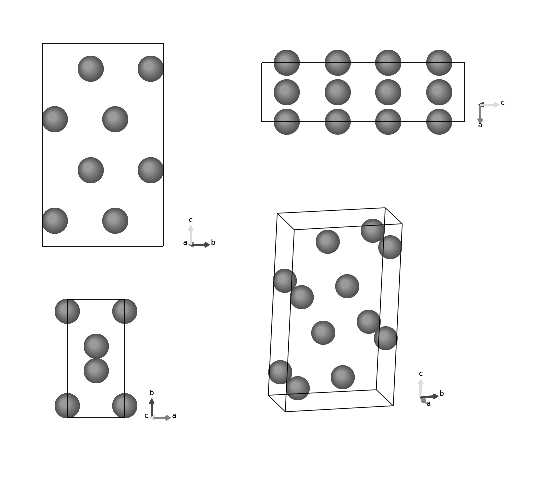
\includegraphics[scale=1.2]{4_image_alphs_greyscale}
\caption{Orthorhombic crystal structure of \textalpha-uranium}
\end{figure}

%The U-Mo alloy has been identified as a high-performance fuel due to its high uranium density and low neutron capture cross-section~\cite{ewh2010microstructural,smirnova2013ternary,rest2009analysis,landa2013density}.


\begin{figure}
\centering
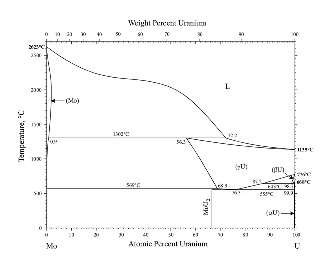
\includegraphics[width=4.5 in]{u-mo-phase-diagram}
\caption[U--Mo phase diagram]{Uranium--Molybdnum phase diagram. Image reprinted with permision from Okamoto~\cite{okamoto2012mo}}
\label{fig:umophase}
\end{figure}

\begin{figure}
\centering
\includegraphics[width=4.25 in]{images/u-al-phase-d.png}
\caption[U--Al phase diagram]{Uranium--Aluminum phase diagram. Image reprinted with permission from Okamoto~\cite{okamoto2012mo}}
\label{fig:ualphase}
\end{figure}



Before the current interest in U--Mo metallic fuel, some of the early nuclear reactors used metallic fuel because of the combination of high uranium density and metallic properties. The Godiva IV pulsed reactors at Los Alamos (initially known as \textit{Lady Godiva}) used U--Mo alloys, which date back to 1960. The Fast Burst Reactor (FBR) at White Sands, the Army Pulsed Radiation Facility (Aberdeen, MD), and the Sandia Pulsed Reactor II also used U--Mo alloys. All of these reactors utilized the \textgamma~phase of uranium, but because of the short irradiation time, the impacts of fuel burnup were minimal~\cite{horak1973operating}. The Dounreay Fast Reactor used a number of metal-fuel-based designs, which inclueds U--9.1Mo (9.1 wt\% Mo) and U--7Mo clad in niobium. The highly alloyed fuel cracked more, even though the U--9.1Mo fuel swelled slightly less than U--7Mo alloy~\cite{cottrell1964development}. In U.S. the Enrico Fermi Fast Breeder Reactor (EFFBR) was the first commercial fast reactor that used U--10Mo fuel. 

The primary concern was to ensure that the fuel would remain in the \textgamma-phase during the operating condition. A series of experiments have been performed to map the fission rate and temperature dependence of the \textgamma-phase's stability~\cite{no20031374}. Two types of U--Mo alloy fuel have been designed and tested. One is monolithic fuel, in which a thin layer of U--Mo foil is bonded to aluminum cladding. The other is a dispersion fuel in which of U--Mo fuel particles are dispersed in an Al matrix.



For five decades, dispersion fuels have powered many test and research reactors worldwide. The manufacturing process and operating conditions are well established for these types of fuels. High-burnup testing of dispersion fuels showed a pattern of \mbox{breakaway} swelling\footnotemark\@ behavior at intermediate burnup. The post-irradiation examination of the U--Mo dispersion fuel revealed that this phenomenon is related to the formation of ternary aluminide phase. Reaction between the U--Mo fuel kernels and aluminum cladding occurs during irradiation and forms a ternary [(U--Mo)Al$_x$] phase which releases the fission gas at the boundary between the interaction phase and the aluminum matrix~\cite{leenaers2004post,jue2014microstructural,van2008transmission, olander2009growth}. These gas bubbles have a tendency to aggregate into the gas pockets, which weakens the fuel meat by exerting internal pressure. The result is mechanical failure and increase in fuel volume. To eliminate the fuel--matrix interaction, a `monolithic' U--Mo fuel was suggested. In monolithic fuels, a zirconium foil is used as a diffusion barrier between the fuel and the cladding (aluminum) to prevent diffusion of molybdenum into the cladding~\cite{jue2014microstructural}.

\footnotetext{\textit{Breakaway} is defined as ``the limiting exposure, beyond which there will be a marked increase in the rate of swelling as a function of burnup~\cite{osti_10163384}"}.



\section{Fission Gas}
The behavior of fission products xenon and krypton has perplexed and fascinated both the experimentalists and theorists more than many processes simultaneously occur in a nuclear fuel element during irradiation. These inert gases are insoluble in fuel matrix, causing them to form small gas bubbles. If the gas is released from the fuel, the pressure within the fuel pin rises and that ultimately results in failure. If the fission gases are retained in the fuel, however, they almost always precipitates as bubbles and causes swelling in the fuel matrix. Swelling adversely impact the fuel efficiency. It impacts the thermal conductivity of the fuel thereby disrupts the efficient heat extraction from the fuel. One particular xenon isotope, $^{135}$Xe has a large neutron absorption cross section which can lead a reactor poisoning. As a result the basic aspects of inert gas behavior were studied for fuel such as UO$_2$.

Xenon is produced directly from fission. 0.3\% of the fission products are $^{135}$Xe. It is also produced by the decay of $^{135}$I via the following scheme:

\begin{equation*}
\ce{^{135}Te ->[$19 \text{s}$] ^{135}I ->[6.7h] ^{135}Xe}
\end{equation*}

$^{135}$I constitutes almost 6.1\% of fission products. Thus, 95\% of the total xenon production is due to the decay of iodine. Xenon is removed from the reactor by a beta decay or by neutron absorption:
\begin{equation*}
\ce{^{135}Xe ->[9.1 $\text{hr}$] ^{135}Cs + $\beta$}
\end{equation*}

In U--Mo fuel fission gas forms bubbles  both inside the grain and in to the grain boundary. In side the grains fission gas forms superlattices~\cite{miller2012advantages, gan2010transmission}. 

This dissertation investigates how fission gas (xenon and krypton) impacts the transport properties of U--Mo fuel. Chapter~2 summarizes theoretical methods used in this work. In Chapter~3, We discuss the reduction of thermal conductivity due to the presence of fission gas. We have used finte element method to approximate the overall thermal conductivity. In Chapter~4, we introduce a new pseudopotential for metallic uranium to study the properties using density functional theory (DFT). In Chapter~5 we look into the diffusion mechanism of xenon in \textgamma-uranium and U--Mo alloy. In Chapter~6, we discuss the conclusions and potential future work.


%In the current work we have investigated how fission gas (xenon and krypton) impacts the U--Mo fuel. In the second chapter we have studied the reduction of thermal conductivity due to the presence of xenon gas. We have implemented finite element method to study the different microstructural configuration of fission gas in U--Mo fuel. In the third chapter we have introduced a new \textit{pseudopotential} for metallic uranium to study the properties using first-principles (Density Functional Theory (DFT)) method. In the fourth chapter we will discuss about the atomistic diffusion mechanism of xenon in U--Mo fuel, which includes the study of xenon gas in the U--Mo fuel using DFT methods. 
















\bibliographystyle{apsrev4-1}
\bibliography{abbreviated,comp}


\include{chapters/xenontherm}

\chapter{Pseudopotential for Plane-Wave Density Functional Theory Studies of Metallic Uranium}
\textit{This chapter was largely published as an article in \textup{Computational Materials \mbox{Science}}. The authors of that article are A. Rafi M. Iasir and Karl D. Hammond of the University of Missouri.}

\section{Introduction}\label{sec_intro}
Uranium is the heaviest naturally-occurring element on Earth. The discovery of
fission in uranium (specifically, in $^{235}$U) impacted not only scientists
and engineers all over the world, it also changed global politics forever. In
nuclear research, the nucleus of the uranium atom is of much more importance
than the electrons surrounding it, but the electronic structure is important
to the thermodynamic properties, including crystal structure. The structural
features are particularly important to the study of next-generation nuclear
fuels, such as \text{U--10Mo}, that are based on metallic uranium.
The electronic behavior of uranium, along with other light actinides (Pa--Pu),
results in a low-symmetry crystal structure at ambient temperature and
pressure---most metallic elements take on relatively high-symmetry structures
(bcc, fcc, and hcp), but the light actinides are either orthorhombic or
monoclinic at standard temperature and pressure~\cite{Soderlind1995}.
Pure uranium exists in three different solid phases at atmospheric pressure,
depending on the temperature:
\textalpha\ (base-centered orthorhombic), \textbeta\ (tetragonal) and
\textgamma\ (body-centered cubic). At atmospheric pressure, \textalpha-uranium
transforms to \textbeta-uranium at approximately 935~K, and \textbeta-uranium transforms to
\textgamma-uranium at approximately
1045~K~\cite{lawson1988structure,akella1997structural}.
The influence of $5f$
electron--electron correlation plays a pivotal role in the crystallographic
behavior of uranium and other light
actinides~\cite{lander2003gh,freemanHandbook1984}; with this in mind, proper
representation of uranium's $5f$ electrons is very important.

The stability of the crystal structures of the inner transition metals has been
the target of several electronic structure studies.
Eriksson and coworkers~\cite{wills1992crystal,eriksson1993first} performed
comparative studies of thorium, protactinium, and uranium's crystal
structures, calculating the equilibrium volume and bulk modulus using the
full-potential linear-muffin-tin-orbital (FP-LMTO) technique and the local
density approximation (LDA)\@.
% ADDED / REPLACED
The predicted equilibrium lattice parameters did not compare well with
experiments.
However, S\"oderlind et al.~\cite{soderlind1994electronic} showed a few years
later that the generalized gradient approximation (GGA) provides much better
agreement with experiment for actinides.

%\textcolor{red}{The calculated lattice parameters and
%equilibrium unit cell volumes showed good agreement with experiments; the
%bulk modulus of protactinium was significantly underestimated, but the values
%for uranium and thorium were within the range of experimental values}.
%
Crocombette \etal~\cite{crocombette2001plane} used norm-conserving
pseudopotentials to study three metallic phases of uranium (\textalpha,
\textgamma, and a hypothetical fcc structure). The calculated equilibrium
volume for \textalpha-uranium was underestimated by more than 6~percent.
S{\"o}derlind~\cite{soderlind2002first} calculated the equilibrium lattice
parameters and also estimated the elastic moduli of
\textalpha-uranium using the FP-LMTO method. The calculated equilibrium
lattice parameters were in good agreement with experimental values, but
the elastic moduli did not agree particularly well with experiments. 
The calculated elastic moduli were likely higher than measured
values because uranium undergoes strong phonon softening with increases in
temperature, and the measured values (taken at room temperature) would
likely be lower than they would be at low
temperatures~\cite{lawson2000melting}.

S\"oderlind's~\cite{soderlind2002first} was the first attempt to calculate
\textalpha-uranium's elastic moduli. Other theoretical studies of light
actinides prior to 2000 using full-core (\ie, non-pseudopotential-based)
techniques are summarized by Jones \etal~\cite{jones2000theoretical}.
Taylor~\cite{taylor2008evaluation} studied uranium phases using the projector
augmented wave (PAW) method~\cite{Bloechl1994} with Perdew and Wang's 1991
(PW91) exchange--correlation functional~\cite{Perdew1992a,Perdew1993}. Taylor
investigated \textalpha, \textgamma, and fcc uranium. The equilibrium lattice
parameters of \mbox{\textalpha-uranium} were within 1\% of experimental
values at 50~K~\cite{barrett1963crystal}. The lattice parameter of
\textgamma-uranium was also in good agreement with measured values, though
the lattice parameter of fcc uranium was overestimated compared to the value
calculated by Crocombette \etal~\cite{crocombette2001plane}. Xiang
\etal~\cite{xiang2008quantum} used the Perdew--Burke--Ernzerhof (PBE) 
exchange--correlation functional~\cite{Perdew1996b,Perdew1997}
to study the equilibrium volume of \textalpha-~and \textgamma-uranium. They
also studied the bct structure, an approximation of the \textbeta~phase.
Their results were also in good agreement with previous full-potential studies
and experiments.
Li \etal~\cite{li2012structure} also studied the
structure, formation energies, and elastic moduli of \textalpha, \textbeta,
\textgamma, fcc, and hcp uranium using the PW91 exchange--correlation
functional~\cite{Perdew1992b}. Their pseudopotential produced reasonably
accurate lattice parameters and cell volumes for
%\textgamma-uranium and
\textalpha-uranium, accompanied by reasonable elastic moduli.
Beeler \etal~\cite{beeler2013first} utilized the PBE
exchange--correlation functional to study uranium, and found similar values
to Li \etal, with the exception of the body-centered tetragonal case
(approximating \textbeta-uranium). The existing pseudopotential
(norm-conserving) in the \textsc{QuantumEspresso} PS library~\cite{pp1,
dal2014pseudopotentials} has a high cut-off energy, making it computationally
expensive to study large supercells. We sought a PAW-based pseudopotential
suitable for studies of uranium alloys.


In the present work, we investigate the crystal structure and elastic
properties of metallic uranium with density functional theory (DFT) with a
projector augmented wave (PAW) pseudopotential~\cite{Bloechl1994}. We
investigate four structures of uranium: \textalpha, \textgamma, bct, and fcc.
Our results are compared with previously-published electronic structure
calculations and experiments. The electronic densities of
states for all four crystal structures are also calculated.
During the development of this pseudopotential, no PAW pseudopotential was available in PS library~\cite{pp1, dal2014pseudopotentials}. However, a PAW pseudopotential (scalar-relativistic) was added recently, so we compare our results with the newly added pseudopotential in the PS library (PsL) for \textalpha- and \textgamma-uranium. We obtain very similar results for \textalpha-uranium, but for \textgamma-uranium, some of the stress--strain curves show discrepancies around the minima. 



\section{Computational Details}\label{sec_comp}
We perform all calculations using density functional theory (DFT) with
plane-wave basis sets as implemented in the software
\textsc{QuantumEspresso}~\cite{giannozzi2009quantum}. We generated a uranium
pseudopotential for use with the Perdew--Burke--Ernzerhof (PBE)
exchange--correlation functional~\cite{Perdew1996b,Perdew1997}.
The projector augmented wave (PAW) pseudopotential-generating software
atompaw~\cite{holzwarth2001projector,tackett2001projector} was used to generate
the PAW pseudopotential for uranium. The same pseudopotential was used for all
subsequent calculations.

The calculations are performed with a scalar-relativistic
model. Full spin--orbit coupling was not used. Previous spin--orbit coupling
results~\cite{soderlind2002first} showed a very small effect on
\textalpha-uranium's equilibrium lattice parameter (within 1\% of
experiment~\cite{barrett1963crystal}). We also have not included on-site
electron correlation (DFT+U) for uranium. S\"oderlind
\etal~\cite{soderlind2014electron} showed that the addition of on-site Coulomb
repulsion leads to a finite magnetization of \textgamma-uranium, which is not
observed in experiments---it is therefore inadvisable to use such corrections.

One of the major challenges in studying actinides using DFT is how to treat the
large number of electrons. The pseudopotential approach effectively reduces the
number of electrons by modeling the ``core'' as a potential energy surface,
so generating a pseudopotential requires one to choose the number of electrons
that will be treated explicitly. There are two approaches common for uranium:
``small-core'' pseudopotentials and ``large-core'' pseudopotentials. In a
large-core pseudopotential, the valence electrons are the $5f$, $6s$, $6p$,
$6d$ and $7s$ shells (14~electrons). In small-core pseudopotentials, the $5s$,
$5p$, and $5d$ shells are also included, which treats 32 electrons as valence
electrons. Iche-Tarrat and Marsden~\cite{iche2008examining} have discussed this
topic and shown that the explicit treatment of 32 electrons only marginally
improves the performance of DFT at significantly higher computational cost.
The valence electron configuration of uranium used when generating our
pseudopotential was $6s^2 6p^6 7s^2 6d^1 5f^3$ (\ie, it is a large-core
pseudopotential).
The radius of the augmentation region was chosen to be 2.5~bohr,
which we determined by starting from half the experimental nearest-neighbor
interatomic distance in \mbox{\textalpha-uranium} and adjusting based on
energy--volume minimization.
The pseudo-partial waves were generated using the RRKJ
scheme~\cite{rappe1990optimized}, which uses a sum of Bessel functions to
represent the pseudo-partial waves.
A plane-wave cutoff energy analysis was performed and a 50~Ry energy cutoff was
found to be sufficient based on a plot of total energy against cutoff energy.
All calculations were performed on primitive cells using the cell geometries
and coordinates given by Crocombette \etal~\cite{crocombette2001plane} for
\textalpha-uranium, Beeler \etal~\cite{beeler2013first} for bct uranium, and
values from the Structure of Crystals database~\cite{StructureofCrystals} for
all other structures.
Periodic boundaries were applied in all directions.
The Monkhorst--Pack scheme~\cite{monkhorst1976special} was used for Brillouin zone
sampling; the $k$-point meshes were $20\times20\times26$, $20\times20\times20$,
$18\times18\times18$, and $20\times20\times20$ for the \textalpha, bct,
\textgamma, and fcc lattices, respectively. A
Methfessel--Paxton~\cite{methfessel1989high} smearing method (width 0.02~Ry)
was used to integrate the bands at the Fermi level.
To calculate the nine unique elastic moduli of orthorhombic \textalpha-uranium,
the energy--strain relationship (see section~\ref{appen_elalpha}) was used as described by Ravindran
\etal~\cite{ravindran1998density}.
For cubic structures, the elastic moduli were evaluated using
volume-conserving orthorhombic and monoclinic distortions  as described by
Beckstein \etal~\cite{beckstein2001first}.

\section{Results}
The pseudopotential itself is generated by
atompaw~\cite{holzwarth2001projector,tackett2001projector}, which takes as
input the augmentation radius ($r_\text{PAW}$), core radius ($r_\text{core}$),
shape function cutoff ($r_\text{shape}$), matching radius ($r_\text{vloc}$),
valence and core electron configurations, density functional, and the
cutoff radii for each of the partial waves ($r_{c,i}$). We assumed
$r_c = r_\text{PAW}$ for all valence electrons except the $6s$ and $7s$
electrons, for which $r_c$ was adjusted. The cutoff radii are given in
Table~\ref{table:pseudopotential}.
These cutoffs, combined with the choice of density functional and valence
electrons, are sufficient to reproduce the pseudopotential in atompaw.
\begin{table}
  \caption[Parameters used to generate the pseudopotential in
    atompaw]{Parameters used to generate the pseudopotential in
    atompaw~\cite{holzwarth2001projector,tackett2001projector}.}
  \label{table:pseudopotential}
  \centering
  \begin{tabular}{l l}
    \toprule
    Cutoff & Value (bohr) \\
    \midrule
    $r_\text{PAW}^{}$   & 2.50 \\
    $r_\text{shape}^{}$ & 2.02 \\
    $r_\text{vloc}^{}$  & 1.50 \\
    $r_\text{core}^{}$  & 1.80 \\
    \midrule
    $r_{c,i}^{}$ & $r_\text{PAW}$ \\
    \multicolumn{2}{l}{\quad EXCEPT} \\
    $r_{c,6s}^{}$       & 1.50 \\
    $r_{c,7s}^{}$       & 1.50 \\
    \bottomrule
  \end{tabular}
\end{table}

\nomenclature{$r_{\text{PAW}}$}{augmentation radius}
\nomenclature{$r_{\text{core}}$}{core radius}
\nomenclature{$r_{\text{shape}}$}{shape function cutoff}
\begin{figure}
	\centering
	%\includegraphics[width=4.3 in]{vol_en_u.eps}
	\includegraphics[width=4.3 in]{vol_en_u.png}
	\caption{Energy vs. volume curve for three different phases of uranium.}
	\label{fig:envsvolu}
\end{figure}

According to our calculations, \textalpha~phase has the lowest energy (see Fig.~\ref{fig:envsvolu}) at ground state. Properties of several uranium phases as calculated with the pseudopotential
presented above are detailed in the rest of this section.


\subsection{\boldmath \textalpha-Uranium} \label{subsec_alphaU}
Uranium's \textalpha\ phase has a base-centered orthorhombic structure with
space group \textit{Cmcm} (no.~63). The asymmetric unit has uranium atoms at
Wyckoff position $4c$ $\Bigl(0, \pm y, \pm\frac{1}{4}\Bigr)$, where the
position parameter $y$ has been found to be a function of
temperature~\cite{barrett1963crystal}.
At room temperature, the value of $y$ has been measured to be
0.1024~\cite{barrett1963crystal,lander1994solid}. There are four atoms in the
standard unit cell (two in the primitive cell).
%(A20 \textit{Strukturbeircht}) designation and oC4 Pearson symbol.
The \textalpha\ phase is thermodynamically favorable at temperatures below
935~K and pressures up to 100~GPa~\cite{le2003structural,akella1997structural}.
This makes the \textalpha\ phase important to the nuclear energy community
because it is the naturally-occurring phase of uranium. The solid-state physics
community also shows interest in \textalpha-uranium because of certain unusual
characteristics, including charge density wave transitions and
superconductivity.

The total energy as a function of unit cell volume for \textalpha-uranium is
shown in Figure~\ref{fig:alpha}; Table~\ref{table:eq_al} summarizes the
optimized lattice parameters, the distance parameter $y$, and the calculated
elastic moduli, along with results from previously-published calculations
and experiments. We confirm that \textalpha-uranium is the lowest-energy crystal
structure among those we tested. Our pseudopotential predicts an equilibrium
volume of 20.49~\AA$^3$, which is in close agreement with the experimental
value of 20.530~\AA$^3$ (at 50~K)\@. The position parameter $y$ exhibits a
minimum-energy 
value of 0.0986 at the equilibrium volume of 20.49~\AA$^3$.
This trend in $y$ is similar to that observed in the calculations of
Wills and Eriksson~\cite{wills1992crystal}.

Our cell volume results differ from previous calculations using
PAW~\cite{beeler2013first}, which obtained an equilibrium volume of
19.987~\AA$^3$ (the work was done using VASP~\cite{kresse1993ab, Kresse1996a, Kresse1996b}). A Murnaghan~\cite{murnaghan1944compressibility} fit to the
total energy as a function of volume for \textalpha-uranium yielded a bulk
modulus of 132.1~GPa, which is larger than the experimental value of
$104 \pm 2$~GPa~\cite{le2003structural},
but agrees closely with the quantum molecular dynamics (QMD) results of
Hood \etal~\cite{hood2008quantum} (133.5 GPa)
and the diamond anvil cell (DAC) experiments of Yoo \etal~\cite{yoo1998phase},
which reported a bulk modulus of 135.5~GPa. Our pseudopotential-based results
are in close agreement with the all-electron FP-LMTO calculations of
S{\"o}derlind~\cite{soderlind2002first}, which gave an equilibrium volume of
20.67~\AA$^3$ and a bulk modulus of 133.0~GPa. A published PAW-based
pseudopotential from Beeler \etal~\cite{beeler2013first} yields an equilibrium
volume of 19.92~\AA$^3$, which is lower than our result and farther from both
the experimental value and the result from all-electron calculations.

\begin{figure}
	\centering
    \includegraphics[width=4.25in]{twoPlots_alphaU}
    \caption[(a)~Calculated total energy as a function of volume for
        \textalpha-uranium. (b)~Calculated total energy as a function of the
        positional parameter $y$ for \textalpha-uranium.]{(a)~Calculated total energy as a function of volume for
        \textalpha-uranium. (b)~Calculated total energy as a function of the
        positional parameter $y$ for \textalpha-uranium. The calculation of $y$
        is constrained to an equilibrium volume of 20.49~\AA$^3$.}
	\label{fig:alpha}
\end{figure}

\begin{sidewaystable} 
%\begin{table}
%\small
%\label{table:eq_al}
\centering
\caption[Ground-state properties and elastic moduli of \textalpha-uranium from present work, compared with the PAW pseudopotential calculations of Beeler]{Ground-state properties and elastic moduli of \textalpha-uranium from present work, compared with the PAW pseudopotential calculations of Beeler \etal~\cite{beeler2013first}, the full-core calculations of S{\"o}derlind~\cite{soderlind2002first}, and experiments from Barrett~\cite{barrett1963crystal}, Le Bihan \etal~\cite{le2003structural}, and Fisher and McSkimin~\cite{fisher1958adiabatic}~(295~K).}
\label{table:eq_al}
%\begin{ruledtabular}
\begin{tabular}{cccccccc}
  \toprule
    & \multicolumn{3}{c}{Theory}
    && \multicolumn{3}{c}{Experiment} \\
    \cline{2-4}\cline{6-8}
				 & present work  & Beeler~\cite{beeler2013first}  & S{\"o}derlind~\cite{soderlind2002first} && Barrett~\cite{barrett1963crystal} & Le Bihan~\cite{le2003structural} & Fisher~\cite{fisher1958adiabatic} \\ \midrule 
$a$ (\AA)		 & 2.834		 & 2.793		 & 2.845	&&	2.836	& 2.8553 & -	\\
$b$ (\AA)		 & 5.862		 & 5.849		 & 5.818	&&	5.867	& 5.8702 & -	\\
$c$ (\AA)		 & 4.932		 & 4.893	     & 4.996	&&	4.936	& 4.9568 & -	\\
$y$ 			 & 0.0986		 & 0.097		 & 0.103	&&	0.102	& 0.102	 & -	\\
volume/atom (\AA$^3$) & 20.48		 & 19.987		 & 20.674	  && 20.535	& 20.770 & -	\\ 
$B$ (GPa)		 & 132.1		 & 151			 & 133		  && -		& 104(2) 	& -	\\
$B'$			 & 5.27			 & -			 & 5.4		  && -		&6.2		& -	\\
$C_{11}$ (GPa)		 & 315			 & 299			 & 300		  &&	-		&-		& 215 \\
$C_{22}$ (GPa)		 & 213			 & 231			 & 220		  &&	-		&-		&199 \\
$C_{33}$ (GPa)		 & 387			 & 364			 & 320		  &&	-		&-		&267 \\
$C_{44}$ (GPa)		 & 135			 &100			 & 150		  &&	-		&-		&124 \\
$C_{55}$ (GPa)		 & 87			 & 150			 & 93		  &&	-		&-		&73 \\
$C_{66}$ (GPa)	     & 104			 & 132			 & 120		  &&	-		&-		&74\\
$C_{12}$ (GPa)		 & 58			 & 59			 & 50		  &&	-		&-		&46\\
$C_{13}$ (GPa)		 & 45			 & 30			 & 5		  &&	-		&-		&22\\
$C_{23}$ (GPa)		 & 146			 & 144			 & 110		  &&	-		&-		&108\\
  \bottomrule
\end{tabular}
%\end{ruledtabular}
%\end{table}
\end{sidewaystable}



The elastic moduli predicted by our pseudopotential are
presented in Table~\ref{table:eq_al}. Like all materials with
orthorhombic symmetry, \textalpha-uranium has nine unique elastic
moduli. Our model overestimates most of the elastic moduli
relative to experiments. The three primary-direction elastic
moduli ($C_{11}$, $C_{22}$, and $C_{33}$) show good agreement
with other theoretical results and with experiment, though all
three principal elastic moduli are overestimated.
The order ($C_{33} > C_{11} > C_{22}$) of these three elastic
moduli is also consistent with experiments. For $C_{55}$ and
$C_{13}$, the present results also show good agreement with
experiments.  The value of $C_{66}$ is overestimated relative to
experiment, but closer than any existing prediction from a
pseudopotential-based calculation. The other elastic moduli are
generally similar to existing theoretical predictions.

\subsection{\textgamma-U: Crystal Structure and Elastic Moduli}
\label{subsec_gamma}

\begin{sidewaystable}
%\label{table_eq_gamma}
\centering
\caption[Equilibrium lattice parameters, volume per atom, and elastic moduli of \textgamma-uranium.]{Equilibrium lattice parameters, volume per atom, and elastic moduli of \textgamma-uranium. Results are compared with the PAW pseudopotential calculations from PsL~\cite{pp1,dal2014pseudopotentials},  Beeler \etal~\cite{beeler2013first}, and Taylor~\cite{taylor2008evaluation}, as well as the norm-conserving pseudopotential calculations of Crocombette \etal~\cite{crocombette2001plane} and the experiments of Wilson and Rundle~\cite{wilson1949structures} at room temperature. Elastic moduli are compared with previous PAW pseudopotential calculations from Beeler \etal~\cite{beeler2013first} and Taylor~\cite{taylor2008evaluation}.}
\label{table_eq_gamma}
%\hspace{-2cm}
%\begin{ruledtabular}
%\footnotesize
\begin{tabular}{ccccccccc}
  \toprule
  & \multicolumn{5}{c}{Theory} && \multicolumn{2}{c}{Experiment} \\
  \cline{2-6}\cline{8-9}
			& present work & PsL~\cite{pp1,dal2014pseudopotentials} & Beeler~\cite{beeler2013first} & Taylor~\cite{taylor2008evaluation} & Crocombette~\cite{crocombette2001plane} && Wilson~\cite{wilson1949structures} & Yoo~\cite{yoo1998phase} \\ \midrule
\rule{0pt}{2.2ex}%  
$a$~(\AA)			&   3.45 & 3.458  & 3.427	& 3.43	 & 3.37		   && 3.47	&-			\\		
volume/atom~(\AA$^3$) & 20.56 & 20.675 & 20.124	& 20.18	 & 19.14	   && 20.89	&-			\\ 
$C_{11}$ (GPa) &	28	& 27   & 86		& 161	 & -	&&-	&-	\\ 
$C_{12}$ (GPa) &	167	& 165  & 155	& 184	 & -	&&-	&-	\\
$C_{44}$ (GPa) &   51	&59	   & 37		& 56	 & -	&&-	&-	\\ 
$B$ (GPa)		&  121	&119   & 132	& 176	 & 170	&&-	& 113.3	\\ \bottomrule
\end{tabular}
%\end{ruledtabular}
\end{sidewaystable}


The structure of \textgamma-uranium at high temperature was first
elucidated by Wilson and Rundle~\cite{wilson1949structures} at Iowa
State University in 1949 using powdered uranium at
800~\textdegree C\@. The \textgamma~phase of uranium has a
body-centered cubic (bcc; Structurbericht designation A2) structure
with two atoms in the standard unit
cell~\cite{yakel1973review,nashchemistry}.
%(space group $Im\overline{3}m$)
It is thermodynamically stable from 1050~K to the melting point of
1406~K~\cite{yoo1998phase}.

In the nuclear fuels community, \textgamma-uranium is preferred to
\textalpha-uranium because it undergoes isotropic thermal expansion
and radiation-induced swelling~\cite{kittel1993history}. 
As Wilson and Rundle observed~\cite{wilson1949structures},
it is not possible to quench pure \textgamma-uranium to room
temperature, but a metastable bcc phase can be retained at room temperature
in U--Mo alloys.
Recently, it was found that the bcc structure can be retained by alloying
uranium with other metals, such as platinum, palladium, niobium, and
zirconium~\cite{kim2016superconductivity}.
In particular, the eutectoid point of \textgamma-uranium with molybdenum
impurities is at approximately 89~weight-percent uranium (see Fig.~\ref{fig:umophase}); to take advantage of
the depressed phase transition temperature (and the associated increase in
stability of the bcc phase), uranium alloyed with 10~wt\% molybdenum
($\approx$\,21.6 at.\%; U-10Mo) is currently being developed as a potential
high-density low-enrichment uranium (LEU) fuel for high-performance research
reactors. The lattice parameters, volume per atom, and elastic moduli as
calculated with our pseudopotential-based model are presented in
Table~\ref{table_eq_gamma}.

The lattice parameters for \textgamma-uranium as calculated with the
pseudopotential presented here are in good agreement with experiments.
The elastic moduli are comparable with those of
Beeler \etal~\cite{beeler2013first} and Taylor~\cite{taylor2008evaluation}.
The value of $C_{12}$ is larger than that of $C_{11}$, which is
a violation of one of the stability criteria for cubic crystals
$(C_{11}-C_{12} > 0)$, often called the Born stability
criterion~\cite{born1940stability,born1954dynamical,Mouhat2014}. This violation
is expected, as the bcc phase of uranium is unstable at low temperatures. The
experimental value of bulk modulus by Yoo \etal~\cite{yoo1998phase} is in good
agreement with our result.

\subsection{Body-Centered Tetragonal Uranium}
\label{subsec_bct}

\begin{table}
%\label{table:eq_bct}
\caption[The optimized lattice parameters (\AA), volume per atom (\AA$^3$) and elastic moduli of bct uranium.]{The optimized lattice parameters (\AA), volume per atom (\AA$^3$), and elastic moduli of bct uranium. Our calculated results are compared with those of Beeler \etal~\cite{beeler2013first}, Li \etal~\cite{li2012structure},
Xiang \etal~\cite{xiang2008quantum}, and S\"oderlind~\cite{Soderlind1998}.}
\label{table:eq_bct}
%\begin{ruledtabular}
\begin{tabular}{cccccc}
  \toprule
		& present work & Beeler~\cite{beeler2013first} & Li~\cite{li2012structure} & Xiang~\cite{xiang2008quantum} & S\"oderlind~\cite{Soderlind1998} \\ \midrule
$a$ (\AA)		&   3.44	   & 3.695	& 3.72 & - & -\\
$c/a$	&	0.8125	   & 0.8	& 1.24 & - & 0.82 \\
vol./atom (\AA$^3$)& 20.44	   & 20.268 & 31.896 & 20.5 & - \\
$C_{11}$ (GPa) &  270		   & 264	& 230 & - & -	\\
$C_{33}$ (GPa) &  257		   & 254	& 204 & - & -	\\
$C_{12}$ (GPa) &  65		   & 55		& 61 & - & -	\\
$C_{13}$ (GPa) &	32		   & 68		& 61 & - & -	\\
$C_{44}$ (GPa) &	59		   & 56		& 79 & - & -	\\
$C_{55}$ (GPa) &	71		   & 56		& 39 & - & - \\
$B$ (GPa)    &	115.4	   & 130	& 114  & - & - \\
  \bottomrule
\end{tabular}
%\end{ruledtabular}
\end{table}
The \textbeta~phase of uranium is stable at atmospheric pressure between 935
and 1045~K~\cite{lawson1988structure}.
Tucker~\cite{tucker1950approximate} determined that it has a tetragonal
structure with 30~atoms per unit cell, but his space group assignment was
later disputed. The assignment of a space group remained a controversy until
1988, when Lawson and coworkers~\cite{lawson1988structure} published neutron
powder diffraction results.
The experimental difficulties lie in the preparation of a single crystal of
\textbeta-uranium and the need to operate at high temperature.
Single crystals of a \textbeta-uranium alloy containing 1.4~atom\% chromium
were created by Tucker~\cite{tucker1951crystal} and quenched to room
temperature, but he did not establish whether this alloy had the same crystal
structure as pure \textbeta-uranium~\cite{lawson1988structure}. An overview of
the development of the crystal structure of \textbeta-uranium is given by
Donohue and Einspahr~\cite{donohue1971structure, donohue1974structures}. The
present consensus is that \textbeta-uranium has a tetragonal crystal structure
with with space group $P4_2/mnm$ (no.~136) and 30~atoms in the unit cell.

We chose to simulate a body-centered tetragonal structure instead of
\textbeta-uranium because of the latter's complexity and computational expense.
A similar simplification was used in studies similar to
ours~\cite{beeler2013first,li2012structure}.
The bct structure has only two atoms per unit cell, and is therefore less
computationally expensive than \textbeta-uranium.
The equilibrium lattice parameters of bct~uranium are presented in
Table~\ref{table:eq_bct}, alongside values from Beeler
\etal~\cite{beeler2013first} and Li \etal~\cite{li2012structure}.
The volume per atom agrees well with Beeler \etal\ but is significantly
different from that of Li \etal.
Xiang \etal~\cite{xiang2008quantum} also studied the bct structure of uranium,
though they did not provide the equilibrium lattice parameter or $c/a$ ratio;
their value of the equilibrium volume per atom was 20.5~\AA$^3$, similar but
larger than our value. Our $c/a$ ratio is in good agreement with
both Beeler \etal~\cite{beeler2013first} (0.8) and
S\"oderlind~\cite{Soderlind1998} (0.82).

\subsection{Face-Centered Cubic Uranium}
\label{subsec_fcc}

\begin{table}
%\label{table:eq_fcc}
\caption[The equilibrium lattice parameter, volume per atom, and elastic moduli
of fcc uranium.]{The equilibrium lattice parameter, volume per atom, and elastic moduli
of fcc uranium. Results are compared with PAW pseudopotential calculations of
Beeler \etal~\cite{beeler2013first}, Taylor~\cite{taylor2008evaluation}, and
Crocombette \etal~\cite{crocombette2001plane}.}
\label{table:eq_fcc}
%\begin{ruledtabular}
\begin{tabular}{cccccc}
  \toprule
				   & present work & Beeler~\cite{beeler2013first} & Taylor~\cite{taylor2008evaluation} & Crocombette~\cite{crocombette2001plane} \\ \midrule
$a$ (\AA)				   & 4.300  		  & 4.433	& 4.48	 & 4.30				\\
volume/atom (\AA$^3$)	   & 21.765   & 21.774	& 22.48  & 19.88			\\ 
$C_{11}$ (GPa) &  	67			& 46	 & 184 &-	  \\
$C_{12}$ (GPa) &	130			& 144	 & 267 &-	  \\
$C_{44}$ (GPa) &	38			& 40	 & 28  &-   \\
$B$ (GPa)		&	108.7		& 111	 & 239	&148	\\
  \bottomrule
\end{tabular}
%\end{ruledtabular}
\end{table}
Face-centered cubic uranium does not exist in nature, but it is a reasonable
way to check the pseudopotential. Beeler \etal~\cite{beeler2013first} and
Taylor~\cite{taylor2008evaluation} studied this structure as well, so we
compare our results with theirs.
Table~\ref{table:eq_fcc} shows the equilibrium parameters and elastic moduli
as calculated with our model and with several other published pseudopotentials.
Our results are in good agreement with other pseudopotential calculations,
particularly those of Beeler \etal~\cite{beeler2013first};
the bulk modulus shows good agreement with their value as well.
It should be noted that $C_{12}$ is still higher than $C_{11}$, confirming that this model predicts the fcc phase to be unstable.

\subsection{Electronic Density of States}
\begin{figure}
	\centering
	\includegraphics[width=4.8in]{total_DOS_allU}
    \caption{Total electronic densities of states of \textalpha, \textgamma,
      bct, and fcc uranium near the Fermi level.}
	\label{fig:totDos}
\end{figure}

\begin{figure}
	\centering
	\includegraphics[width=4.8in]{spdf_orbital}
    \caption[The partial electronic densities of states of \textalpha,
      \textgamma, bct, and fcc uranium near the Fermi level.]{The partial electronic densities of states of \textalpha,
      \textgamma, bct, and fcc uranium near the Fermi level. The $6d$ (blue
      line) and $5f$ (black line) electronic orbitals are shown. The $s$ (red)
      and $p$ (green) electronic orbitals are also included, but due to their
      very low contributions near the Fermi level, they are barely visible.}
	\label{fig:fdorbitals}
\end{figure}

The electronic densities of states (DOS) of \textalpha, bct, \textgamma, and
fcc uranium are shown in Figure \ref{fig:totDos}. The partial densities of
states for the $5f$ and $6d$ orbitals are shown in Figure~\ref{fig:fdorbitals}.
We have only shown the partial densities of states for the $5f$ and $6d$
orbitals because these are the dominant orbitals near the Fermi level of
uranium. There are also contributions from $6s$, $6p$, and $7s$ orbitals near
the Fermi level, but these contributions are not as significant as the dominant
$5f$ and $6d$ orbitals.
%At the Fermi level, the dominant electronic contributions are from the $5f$
%orbitals, though the $6d$ orbitals do contribute.
Electrons near the Fermi level
are important because they are responsible for most of the metallic behavior.
From Figure~\ref{fig:totDos}, it can be seen that the DOS spreads over energies
between $-4$~eV and 2~eV relative to the Fermi level. The density of states
with our model is comparable to those calculated by Beeler
\etal~\cite{beeler2013first} and Xiang \etal~\cite{xiang2008quantum}.
For bcc and bct uranium, the $f$ orbitals spread over a broader range of
energies near the Fermi level and show multiple peaks above the Fermi level.
The high density of states at energies above the Fermi level in the bct
and \textgamma\ phases suggests that these phases would be favored over
\textalpha-uranium at high temperature.

\section{Conclusion}
The equilibrium structures, cell volumes, and elastic moduli have been
calculated using DFT with a newly-parameterized pseudopotential model for four
different uranium phases (\textalpha, \textgamma, body-centered
tetragonal, and face-centered cubic). Our results are either in good agreement
with previous work or show improvement in comparison with experiments.
Studying pure uranium is the first step in exploring different alloys of
uranium that are of interest to the nuclear fuels community.
Due to the lower cutoff energies that can typically be used, PAW-based
pseudopotentials allow one to study larger supercells, which in turn provide
more accurate studies of vacancy formation, grain boundaries, and fission gas
transport.

According to our pseudopotential, \textalpha-uranium is the lowest-energy
crystal structure of the ones tested.
The calculated elastic moduli show good agreement with previous DFT studies
and experiments. Our model shows good agreement with previous pseudopotentials,
but generally provides results that are either comparable to previously
published pseudopotentials or closer to experimental values than previously
published pseudopotentials.
The three elastic moduli associated with shear ($C_{44}$, $C_{55}$, and
$C_{66}$) show better agreement with experimental results than the tensile
components. The lattice parameters of the bct structure are also very similar
to those predicted by Beeler \etal~\cite{beeler2013first}, but they deviate
significantly from those of Li \etal~\cite{li2012structure}.
The elastic moduli show very similar trends to previously-published models,
apart from $C_{23}$, which is over-predicted by our model.

For \textgamma-uranium, which is of great interest for the development of
low-enrichment uranium fuel, the lattice parameters are in close agreement with
those of of Taylor \etal~\cite{taylor2008evaluation} and with experiments.
Apart from the elastic modulus $C_{11}$, the values of all computed parameters
show very little discrepancy compared with those from the work of Taylor
\etal~\cite{taylor2008evaluation} and Beeler \etal~\cite{beeler2013first}.
The bulk modulus shows very good agreement with experiment.

For fcc uranium, a hypothetical crystal structure, the computed lattice
parameter is in close agreement with values reported by Beeler
\etal~\cite{beeler2013first} and by Crocombette
\etal~\cite{crocombette2001plane}. The equilibrium volume per atom does show a
discrepancy from Crocombette but is in good agreement with Beeler \etal.
The elastic modulus $C_{44}$ is also in good agreement with Beeler \etal,
whereas $C_{11}$ is intermediate between the value predicted by Beeler \etal\
and that predicted by Taylor \etal.
Lastly, the electronic density of states shows that the $5f$
orbital partial density of states is the largest contribution to the total
density of states at the Fermi energy, and the $5f$ electrons therefore
contribute the most to the bonding and conductivity of uranium. Most of the
$5f$ orbital electron density is spread over energies between $-4$ and 2~eV
relative to the Fermi level. We also find that \textgamma-uranium has the
highest density of states at energies above the Fermi level, confirming that it
should be favored at high temperature.

%\appendixname
\newpage
\addcontentsline{toc}{section}{\protect\numberline{}Appendix: Elastic Parameter Calculation of \textalpha-uranium}\label{appen_elalpha}
\section*{Appendix: Elastic Parameter Calculation of \boldmath $\alphaup$-uranium}
In this appendix, we will discuss the stress-strain relationships that were used to calculate the nine independent elastic constants of \textalpha-uranium. The base-centered orthorhombic phase of uranium has three lattice parameters: $a$, $b$, and $c$; with the Bravais lattice matrix
\begin{equation}\label{eq_lattic_alphaU}
\mathbf{R} = \begin{bmatrix}
			\frac{a}{2} & -\frac{b}{2} & 0 \\
			\frac{a}{2} & \frac{b}{2} & 0 \\
			0			&    0        & c 
			\end{bmatrix}.
\end{equation}
Applying a small strain to the equilibrium lattice changes the total energy, and from this information, the elastic parameters are deduced. The elastic parameters are identified as proportional to the second order coefficient in a polynomial fit of the total energy as a function of the distortion parameter $\delta$~\cite{wallace1998thermodynamics}. The distortion of the lattice vectors follows the rule $\mathbf{R'}=\mathbf{RD}$. Here, $\mathbf{R'}$ is a matrix containing the components of the distorted lattice vectors and $\mathbf{D}$ is the symmetric distortion matrix.



The internal energy of a crystal under strain $\delta$ can be expanded in powers of the strain tensor with respect to initial energy of the unstrained crystal in the following way:
	\begin{equation}
	\label{eq_taylor_el}
	E(V,\delta) = E(V_0,0) + V_0 \left ( \sum_i \tau_i \xi_i d_1 + 1/2 \sum_{ij} C_{ij} \delta_i \xi_i \delta_j \xi_j \right ) + \mathcal{O}(\delta^3) 
	\end{equation}
The unstrained volume is $V_0$, and $E(V_0,0)$ is the energy of the unstrained system. Voight notation has been used in Eqn.~\eqref{eq_taylor_el} (\ie, $xx$, $yy$, $zz$, $yz$, $xz$, and $xy$, respectively, are replaced with 1--6). Here, $yz$, $xz$, and $xy$, are equal to $zy$, $zx$, and $yx$, and for this reason, $\xi_i$ is equal to 1 for $i=1$, $2$, and $3$ and equal to $2$ for $i=4$, $5$, and $6$. $\tau_i$ is a component of the stress tensor. The first three elastic constants; $C_{11}$, $C_{22}$, and $C_{33}$; are obtained form the following distortions:
\begin{equation}
\label{eq_D1}
	\mathbf{D_1} =  \begin{bmatrix}
						1+\delta & 0 & 0 \\
						0 & 1 & 0 \\
						0 & 0 & 1 \\
						\end{bmatrix}
\end{equation}

\begin{equation}
\label{eq_D2}
	\mathbf{D_2} = \begin{bmatrix}
						1 & 0 & 0 \\
						0 & 1+\delta & 0 \\
						0 & 0 & 1 \\
					\end{bmatrix}
\end{equation}

\begin{equation}
\label{eq_D3}
\mathbf{D_3} =  \begin{bmatrix}
						1 & 0 & 0 \\
						0 & 1 & 0 \\
						0 & 0 & 1+\delta \\
						\end{bmatrix}.
\end{equation}
The internal energies for these three distortions can be obtained from 
\begin{equation}
\label{eq_d1d2d3}
E(V,\delta) = E(V_0,0) + V_0\tau_i \delta + \frac{V_0C_{ii}\delta^2}{2}.
\end{equation}
The constants $C_{44}$, $C_{55}$, and $C_{66}$ are related to the distortions:
\begin{equation}
\label{eq_D4}
	\mathbf{D_4} = \begin{bmatrix}
						\frac{1}{(1-\delta^2)^{1/3}} & 0 & 0 \\
						0 & \frac{1}{(1-\delta^2)^{1/3}} & \frac{\delta}{(1-\delta^2)^{1/3}} \\
						0 & \frac{\delta}{(1-\delta^2)^{1/3}} & \frac{1}{(1-\delta^2)^{1/3}} \\
						\end{bmatrix}
\end{equation} 

\begin{equation}
\label{eq_D5}
	\mathbf{D_5} =  \begin{bmatrix}
						\frac{1}{(1-\delta^2)^{1/3}} & 0 & \frac{\delta}{(1-\delta^2)^{1/3}} \\
						0 & \frac{1}{(1-\delta^2)^{1/3}} & 0 \\
						\frac{\delta}{(1-\delta^2)^{1/3}} & 0 & \frac{1}{(1-\delta^2)^{1/3}} \\
						\end{bmatrix}
\end{equation}
and
\begin{equation}\label{eq_D6}
						\mathbf{D_6} = \begin{bmatrix}
						\frac{1}{(1-\delta^2)^{1/3}} & \frac{\delta}{(1-\delta^2)^{1/3}} & 0 \\
						\frac{\delta}{(1-\delta^2)^{1/3}} & \frac{1}{(1-\delta^2)^{1/3}} & 0 \\
						0 & 0 & \frac{1}{(1-\delta^2)^{1/3}} \\
						\end{bmatrix}.
\end{equation}	
These three elastic constants can be calculated from the corresponding internal energy:
\begin{equation}
							E(V,\delta) = E(V_0,0) + V_0\tau_i \delta + \frac{V_0C_{ii}\delta^2}{2}
\end{equation}
The last three distortions are
\begin{equation}\label{eq_D7}
						\mathbf{D_7} = \begin{bmatrix}
						\frac{1+\delta}{(1-\delta^2)^{1/3}} & 0 & 0 \\
						0 & \frac{1-\delta}{(1-\delta^2)^{1/3}} & 0 \\
						0 & 0 & \frac{1}{(1-\delta^2)^{1/3}} \\	
						\end{bmatrix}
\end{equation}			

\begin{equation}\label{eq_D8}
						\mathbf{D_8} =  \begin{bmatrix}
						\frac{1+\delta}{(1-\delta^2)^{1/3}} & 0 & 0 \\
						0 & \frac{1}{(1-\delta^2)^{1/3}} & 0 \\
						0 & 0 & \frac{1-\delta}{(1-\delta^2)^{1/3}} \\
						\end{bmatrix}
\end{equation}	
and
\begin{equation}\label{eq_D9}
						\mathbf{D_9} = \begin{bmatrix}
						\frac{1}{(1-\delta^2)^{1/3}} & 0 & 0 \\
						0 & \frac{1+\delta}{(1-\delta^2)^{1/3}} & 0 \\
						0 & 0 & \frac{1-\delta}{(1-\delta^2)^{1/3}} \\	
						\end{bmatrix}
\end{equation}
The internal energies related to these three distortions are given by the following equations:
\begin{gather}
E(V,\delta) = E(V_0, 0) + V_0\left [ \tau_1 - \tau_2 \right ] \delta + \frac{1}{2} \left(C_{11} + C_{22} -2C_{12}  \right)\delta^2 \\
E(V,\delta) = E(V_0, 0) + V_0\left [ \tau_1 - \tau_3 \right ] \delta + \frac{1}{2} \left(C_{11} + C_{33} -2C_{13}  \right)\delta^2 \\
E(V,\delta) = E(V_0, 0) + V_0\left [ \tau_2 - \tau_3 \right ] \delta + \frac{1}{2} \left(C_{22} + C_{33} -2C_{23}  \right)\delta^2
\end{gather}
The above equations can be used to calculate the remaining elastic constants $C_{12}$, $C_{13}$, and $C_{23}$\@. The energy and strain relations are calculated and included in Figures~\ref{fig_D123}, \ref{fig_D456}, and \ref{fig_D789}\@. 

\begin{figure}
	\centering
	\includegraphics[]{d123_alphaU.eps}
	\caption{Changes in the strain energy as a function of strain using distortion matrix~$D_1$~\eqref{eq_D1}, $D_2$~\eqref{eq_D2}, and $D_3$~\eqref{eq_D3}.}
	\label{fig_D123}
\end{figure}

\begin{figure}
	\centering
	\includegraphics[]{d456_alphaU.eps}
	\caption{Changes in the strain energy as a function of strain using distortion matrix~$D_4$~\eqref{eq_D4}, $D_5$~\eqref{eq_D5}, and $D_6$~\eqref{eq_D6}.}
	\label{fig_D456}
\end{figure}

\begin{figure}
	\centering
	\includegraphics[]{d789_alphaU.eps}
	\caption{Changes in the strain energy as a function of strain using distortion matrix~$D_7$~\eqref{eq_D7}, $D_8$~\eqref{eq_D8}, and $D_9$~\eqref{eq_D9}.}
	\label{fig_D789}
\end{figure}

\clearpage
\addcontentsline{toc}{section}{\protect\numberline{}Appendix: Elastic Parameter Calculation for \textgamma-uranium}\label{appen_bccel}

\section*{Appendix: Elastic Parameter Calculation for \boldmath \textgamma-uranium}
Applying a small strain ($\delta$) to the equilibrium lattice changes the total energy, and from this information, the elastic parameters are deduced. The distortion of a lattice vector follows the rule $\mathbf{R'} = \mathbf{RD}$. Here, $\mathbf{R}$ is the Bravais lattice vector, $\mathbf{R'}$ is a matrix containing the components of the distorted lattice vectors, and $\mathbf{D}$ is the symmetric distortion matrix.


By symmetry, there are only three independent elastic parameters for a cubic system (\ie, $C_{11}, C_{12}$, and $ C_{44}$).
Elastic parameters are evaluated from the total energy of the crystal, to which volume-conserving orthorhombic $[C'=(C_{11} - C_{12})/2]$ and monoclinic $(C_{44})$ distortions are applied. The relevant distortion matrices are 
%\[\begin{bmatrix}
\begin{equation}
\mathbf{D_\text{ortho}} = \label{eq:ortho}
		\begin{bmatrix}
		1+\delta_o & 0 & 0 \\
		0 & 1-\delta_o & 0 \\
		0 & 0 & \frac{1}{1-\delta_o^2}\\
		\end{bmatrix}
\end{equation}
%\end{bmatrix} \]
and
\begin{equation}
\label{eq:mono}
\mathbf{D_\text{mono}} = \begin{bmatrix}
	1 & \delta_m & 0 \\
	\delta_m & 1 & 0 \\
	0 & 0 & \frac{1}{1-\delta_m^2} \\
\end{bmatrix}.
\end{equation}
The associated total energy change for an orthorhombic distortion is 
\begin{equation}
\label{eq_ortho}
\Delta E = V(C_{11} - C_{12})\delta_o^2 + \mathcal{O}(\delta_o^4) .
\end{equation}
For a monoclinic distortion, the energy change is
\begin{equation}
\label{eq_mono}
\Delta E = 2VC_{44}\delta_m^2 + \mathcal{O}(\delta_m^4).
\end{equation}

\begin{figure}
	\centering
	\includegraphics[width=4.25 in]{figure_bulk}
    \caption[Energy as a function of lattice parameter for \textgamma-uranium]{Energy as a function of lattice parameter for \textgamma-uranium. (a)~this work with a $k$-point mesh of $30\times30\times30$; (b)~Pseudopotential from PS library~\cite{dal2014pseudopotentials, pp1}
 with a $k$-point mesh of $30\times30\times30$; (c)~Pseudopotential from PS library~\cite{dal2014pseudopotentials, pp1}
 with $42\times42\times42$ $k$-point mesh.}
	\label{fig:bulkgamma}
\end{figure}

\begin{figure}
	\centering
	\includegraphics[width=4.25 in]{figure_mono}
    \caption[Changes in the strain energy as a function of strain $(\delta)$ for monoclinic distortions of \textgamma-uranium]{Changes in the strain energy as a function of strain $(\delta)$ for monoclinic distortions of \textgamma-uranium (Eq.~\eqref{eq:mono} and Eq.~\eqref{eq_mono}). (a)~this work; (b)~Pseudopotential from the PS library~\cite{dal2014pseudopotentials, pp1}. Increasing the number of $k$-points does not improve the smoothness of plot (b).}
\label{fig:monogamma}
\end{figure}

\begin{figure}
	\centering
	\includegraphics[width=4.25 in]{figure_ortho}
    \caption[Changes in the strain energy as a function of strain $(\delta)$ for orthorhombic distortions of \textgamma-uranium]{Changes in the strain energy as a function of strain $(\delta)$ for orthorhombic distortions of \textgamma-uranium (Eq.~\eqref{eq:ortho} and Eq.~\eqref{eq_ortho}). (a)~this work; (b)~Pseudopotential from the PS library~\cite{dal2014pseudopotentials, pp1}.}
	\label{fig:orthogamma}
\end{figure}



\clearpage
\bibliographystyle{apsrev4-2}
\bibliography{abbreviated,final}
%\bibliography{abbreviated,pseudo}


\chapter{Conclusions and Future Work}
Things to cover here in the future work.

\begin{itemize}
	\item How can I improve the model for thermal conductivity model.
	\item Can include grain boundary growth. Can through in a swelling model.
	\item Studying the stability of U--Mo alloy with respect to temperature, which can be studied using ab initio molycular dynamcis.
	\item Collecting all the rate limiting steps of xenon diffusion in u--mo alloys.
	\item Come up with a kinetic Monte Carlo Method.
	\item Improve the model somehow , I don't know how.


\end{itemize}



\bibliographystyle{unsrt}
\bibliography{abbreviated,comp}







\appendix
%\chapter{FEM Discretization of the heat equation}\label{appen_discretize}

The divergence theorem in vector calculus can be stated as follows. Let $V$ be region in space with boundary $\partial V$. Then the volume integral of the divergence $\nabla \cdot \mathbf{F}$ over $V$ and the surface integral of $\mathbf{F}$ over the boundary $\partial V$ of $V$ are related by
\begin{equation}
\label{eq_divergence}
\int_V \left ( \nabla \cdot \mathbf{F}  \right) dV = \int_{\partial V} \mathbf{F}\cdot d\mathbf{a}
\end{equation} 
A special case of divergence theorem follows by specializing the plane. Letting $S$ be a region in the plane with boundary $\partial S$, then Eqn~\ref{eq_divergence} can be written in the following ways
\begin{equation}
\label{eq_div_plane}
\int_S \nabla \cdot \mathbf{F}dA = \int_{\partial S} \mathbf{F}\cdot \hat{n} ds
\end{equation}
It turns volume integral into a surface integral. Multiplying Eqn~\ref{eq_div_plane} with a smooth function $\Upsilon$ and integrating  
\begin{equation}
\label{eq_test_func}
\int_S \Upsilon\left ( \nabla\cdot \mathbf{F} dA  \right) = \int_S \nabla \cdot \left(\Upsilon \mathbf{F} \right)dA - \int_S \nabla \Upsilon\cdot \mathbf{F}dA 
\end{equation}
Using the divergence theorem~\ref{eq_div_plane} the above equation can be written in the following way:
\begin{equation}
\int_S \Upsilon\left ( \nabla\cdot \mathbf{F} dA  \right) = \int_{\partial S}\Upsilon \mathbf{F} \cdot \hat{n} ds  - \int_S \nabla \Upsilon\cdot \mathbf{F}dA 
\end{equation}
In the finite element calculation, for example $\mathbf{F}=-K(x)\nabla u$, and with the help of divergence theorem the weak form equation becomes
\begin{equation}
-\int_{S} \Upsilon\left(\nabla \cdot K(x) \nabla u \right ) dA = \int_{S} \nabla \Upsilon \cdot K(x) \nabla u dA - \int_{\partial S} \Upsilon \left( K(x) \nabla u\cdot \hat{n}  \right) ds 
\end{equation}
Using the inner product notation the above integral equation can be represented as follows:
\begin{equation}
-\left( \Upsilon, \nabla\cdot K(x) \nabla u \right ) = \left ( \nabla \Upsilon, K(x) \nabla u \right ) - \langle \Upsilon, K(x) \nabla u\cdot \hat{n}\rangle
\end{equation}
To approach the problem numerically the term $ \langle \Upsilon, K(x) \nabla u\cdot \hat{n}\rangle$ is usually handed by boundary condition, and the term $ \left ( \nabla \Upsilon, K(x) \nabla u \right )$  needs to be solve iteratively.
%something

%\chapter{Orthogonal Plane Wave}\label{appen_opw}

For now, we will try to approximate the time-independent \schrod equation so that we can achieve self-consistency. Let $V(r)$ be the potential seen by each electron. Then each energy eigenfunction will satisfy the following equation:
\begin{equation}
\label{eigeqn}
\hat{\mathcal{H}}\psi_i = \left[\hat{T}+\hat{V}(r)\right]\psi_i = E_i\psi_i 
\end{equation}
Here, $\hat{T}$ is the kinetic energy operator ($-\hbar^2\nabla^2/2m$), and $E_i$ is the energy of the $i$-th state. The next step is to distinguish between the core and the valence state. The index $\alpha$ will be used for the core electrons and $v$ will be used for the valence band. The core states are the same as in the isolated ion, but their energies are different (\ie, $E_\alpha$, is different):
\begin{equation}
\label{eq_eigalpha}
\left[\hat{T}+\hat{V}(r)\right]\psi_\alpha = E_\alpha \psi_\alpha
\end{equation}
Here, the subscript $\alpha$ not only denotes the position of the ion but also the energy and angular momentum quantum numbers of the state in the equation. This is a well-defined Sturm--Liouville eigenvalue problem, apart from not knowing $V(r)$. We can approach the problem in several ways. The most common is to represent $\psi_{\alpha}$ by a basis set. Plane-wave basis sets are often used in band structure calculations. If we expand the \schrod Eqn.~\eqref{eq_eigalpha} with a complete set of states,  then we may obtain a linear solution of simultaneous equations in the expansion coefficients. The problem of  solving differential equations then becomes a matrix diagonalization problem. 

The choice of plane waves has its pros and cons. One of the difficulties of using plane waves is that, it typically requires a large number of plane waves to give a reasonable description of the wavefunction. Thus the solution becomes very difficult. In addition the core electrons have higher kinetic energy near the nucleus (see Fig.~\ref{fig_hydrogen}), which makes it even harder for plane waves to approximate those electrons. Herring~\cite{herring1940new} suggested that, rather than expanding the valence electron wave function in plane waves, a more rapidly convergent procedure is to expand in \textit{orthogonalized} plane waves (OPWs). Hopefully, the expansions in terms of OPWs, would require fewer terms and therefore yield a faster calculation. The OPWs with wave number $\mathbf{k}$ can be defined as follows:
\begin{equation}
\label{eq_opw}
OPW_{\vb{k}} = e^{i\vb{k\cdot r}} - \sum_{\alpha} \psi_{\alpha}(\vb{r}) \psi^{\ast}_{\alpha} e^{i{\vb{k\cdot r}}} d \vb{r}
\end{equation}

An example would be sodium, which has a ground state configuration of $1s^2 2s^2 2p^6 3s^1$. The core orbitals would be $1s^2 2s^2 2p^6$. For so-called simple metals (\ie, Na, Mg, and Al), the electron wavefunction is rapidly convergent in the OPW basis. Before going any further, let's check whether this OPW (\ref{eq_opw}) is orthogonal to the core states. Let's assume an arbitrary core wavefunction $\psi_{\beta}$ and check the orthogonality with \ref{eq_opw}:
\begin{equation}
\int\psi^{\ast}_{\beta}(\vb{r})OPW_{\vb{k}}d\vb{r} = \int \psi^{\ast}_{\beta} (\vb{r}) e^{i\vb{k\cdot r}} d\vb{r} - \sum_{\alpha} \delta_{\alpha\beta} \int \psi^{\ast}_{\alpha} (\vb{r}) e^{i\vb{k\cdot r}} d\vb{r} = 0 
\end{equation}
It is convenient to normalize the plane waves in the unit cell volume of the metal $\Omega$, and we will use Dirac's bra-ket notation for the wave functions from now on. The plane wave becomes
\begin{equation}
	\ket{\vb{k}} = \Omega^{-1/2}e^{i\vb{k\cdot r}}
\end{equation}
For core electron wave functions
\begin{equation}
	\ket{\alpha} \equiv \psi_{\alpha} (\vb{r}) 
\end{equation}
where $\bra{\alpha} = \ket{\alpha}^{\ast}$, and
\begin{equation}
	\braket{\alpha}{\vb{k}} = \Omega^{-1/2} \int \psi^{\ast}_{\alpha} (\vb{r}) e^{i\vb{k\cdot r}} d\vb{r}
\end{equation}
Thus the OPW equations becomes
\begin{equation}
	OPW_{\vb{k}} = \ket{\vb{k}} - \sum_{\alpha} \ket{\alpha}\braket{\alpha}{\vb{k}}
\end{equation}
The projection operator $P$ can be defined as follows:
\begin{equation}
\label{eq_proj}
P = \sum_{\alpha} \dyad{\alpha}{\alpha}.
\end{equation}
The $P$ operator projects any function onto the core states. In terms of the $P$ operator the OPW can take following form:
\begin{equation}
	OPW_{\vb{k}} = (1-P)\ket{\vb{k}}.
\end{equation}
Now, we can expand the valence-band (valence electron) state as a linear combination of  OPWs:
\begin{equation}
	\psi_{k} = \sum_q a_q (\vb{k})(1-P)\ket{\vb{k}+\vb{q}}
\end{equation}
Before going a bit further, lets see how kinetic energy is represented by plane waves.
\begin{equation}
\label{eq_kin}
	\bra{q'}-\frac{\hbar^2}{2m}\nabla^2\ket{q} = \frac{1}{2}\frac{\hbar^2}{2m} \abs{\vb{q}}^2 \delta_{qq'}
\end{equation}
In the above approximation of kinetic energy we assumed the normalizing factor is one.
Now we are going to expand \ref{eq_eigalpha} with OPWs, and the \schrod equation becomes
\begin{equation}
\hat{\mathcal{H}}\psi_k = \sum_q a_q (\vb{k})\hat{\mathcal{H}}(1-P)\ket{\vb{k}+\vb{q}}=E_k\sum_q a_q (\vb{k}) (1-P) \ket{\vb{k}+\vb{q}}
\end{equation}
where $\hat{\mathcal{H}}$ consists both the kinetic energy and the potential energy. Multiplying on the left by $\bra{\vb{k}+\vb{q}'}$, and using Equation~\eqref{eq_kin} we obtain
\begin{multline}
\label{eq_opwd}
a_{q'} (\vb{k}) \frac{\hbar^2}{2m}\abs{\vb{k}+\vb{q}'}^2 + \sum_q a_q (\vb{k})[\bra{\vb{k}+\vb{q}'}V\ket{\vb{k}+\vb{q}} - \sum_{\alpha} E_{\alpha} \braket{\vb{k}+\vb{q}'}{\alpha}\braket{\alpha}{\vb{k}+\vb{q}}]
	= \\
 [a_{q'} (\vb{k}) - \sum_q a_q (\vb{k}) \bra{\vb{k}+\vb{q}'}P\ket{\vb{k}+\vb{q}}]E_{\vb{k}}  
\end{multline}
The above equation can be solved by diagonalizing some of matrix element. If we can evaluate some of the various matrix elements (integrals), we obtain a set of linear algebraic equations.


\bibliographystyle{apsrev4-2}
\bibliography{abbreviated,final}
%\bibliography{abbreviated,other} 


%\chapter{Projector Augmented Wave}\label{appen_paw}

Pseudopotential technique has been proven to be accurate for a large variety of systems, but there is no strict gurantee that it will produce the same results as an all-electron calculation. The challenge with norm-conserving pseudopotentials is that it limits the \textit{softness}. Another way to say it, it needs higher cut-off energy. In the plane-wave basis set for the pseudo wavefunctions is defined by the shortest wave lentgh $\lambda=2\pi/\abs{\vec{G}}$, where $\vec{G}$ is the wave vector. Projector augmented waves (PAW) introduces projectors and auxiliary localized functions to increase the softness of the pseudopotential, at the same time keeping full wave function. In this section I will try to introduce PAW with some basic formalism. The origin of the PAW method lies a transformation that maps the true wavefunctions with their complete nodal structure into auxiliary wavefunctions. The purpose of this transformation is to have a smooth auxiliary wavefunctions, which have a rapidly convergent plane-wave expansion. The PAW method was first proposed by Bl\"ochl in 1994~\cite{blochl1994projector}. The linear transformation is as follows.
\begin{equation}
\ket{\Psi_n} = \hat{\mathcal{T}}\ket{\tilde{\Psi}_n}
\end{equation}
Where, $\ket{\Psi_n}$ is the true all-electron KS single particle wave function, $\ket{\tilde{\Psi}_n}$ is auxiliary smooth wave function, and $\hat{\mathcal{T}}$ is a linear transformation operator. Since the true wave functions are already smooth at a certain minimum distance from the core, $\tilde{\mathcal{T}}$ should only modify the wave function close to the nuclei. Thus the transformation operator becomes
\begin{equation}
\tilde{\mathcal{T}} = 1 + \sum_a \tilde{\mathcal{T}^a}
\end{equation}
Where a is an atom index, $\tilde{\mathcal{T}^a}$, has no effect outside a certain atom-specific augmentation region, $r_C^a$. Inside the augmentation spheres, the true wave function can be expanded in the partial waves $\phi_i^a$, for a corresponding auxiliary smooth partial wave can be defined as $\tilde{\phi}_i^a$, and they connected by the following relation.
\begin{equation}
\label{eq_aug_t}
\ket{\phi_i^a} = (1+\hat{\mathcal{T}}^a)\ket{\tilde{\phi}_i^a} \Rightarrow  \hat{\mathcal{T}}^a \ket{\phi_i^a} = \ket{\phi_i^a} - \ket{\tilde{\phi}_i^a}
\end{equation} 
Here $a$ is an atom index, $i$ comes from partial waves. Outside the augmentation sphere, the partial wave and its smooth counterpart should be identical.
\begin{equation}
\phi_i^a(\mathbf{r}) = \tilde{\phi}_i^a(\mathbf{r}),\  for \quad r > r_c^a
\end{equation} 
Where $\phi_i^a(\mathbf{r})=\braket{\mathbf{r}}{\phi_i^a}$, and similar for $\tilde{\phi}_i^a$. If the smooth partial waves form a complete set inside the augmentation sphere, we can expand the smooth all electron wave functions as 
\begin{equation}
\ket{\tilde{\Psi}_i^a} = \sum_i P_{ni}^a \ket{\tilde{\phi}_i^a}, \quad \abs{\mathbf{r}-\mathbf{R}} < r_c^a
\end{equation}
Where, $P_{na}^a$ are expansion coefficients, and need to be determined. And also, the index a stands for atomic sites, i to dintinguish different partials waves and n connected to quantum numbers $(l,m)$. Since the transformation operator connects the smooth pseudo wave function to true wave function.
\begin{equation}
\ket{\Psi_n} = \hat{\mathcal{T}} \ket{\tilde{\Psi}_n} = \sum_i P_{ni}^a \ket{\psi_i^a}, \quad \abs{\mathbf{r}-\mathbf{R}} < r_c^a
\end{equation} 
Something really interesting about the above equation, the true wave function has the same expansion coefficient $(P_{ni}^a)$ as the pseudo wavefucntion. The transformation operator $\hat{\mathcal{T}}$ is required to be linear, the coefficient must be linear functionals of $\ket{\tilde{\Psi}_n}$, i.e.
\begin{equation}
P_{ni}^a = \braket{\tilde{p}_i^a}{\tilde{\Psi}_n}
\end{equation}
Where $\ket{\tilde{p}_i^a}$ are some fixed functions termed smooth projector functions. As there is no overlap between the augmentation spheres, we expect the smooth all electron wave function, $\ket{\tilde{\Psi}_n^a} = \sum_i \ket{\tilde{\phi}_i^a} \braket{\tilde{p}_i^a}{\tilde{\Psi}_n}$. The projectors have to be localized within an augmentation region
\begin{equation}
\label{eq_paw_complete}
	\sum_i \dyad{\tilde{\phi}_i^a}{\tilde{p}_i^a} = 1
\end{equation}
This also implied that
\begin{equation}
	\braket{\tilde{p}_{i_1}^a}{\tilde{\phi}_{i_2}^a} = \delta_{i_1,i_2},\quad for \quad < r_c^a
\end{equation}
the projector functions should be orthonormal to the smooth partial waves inside the augmentation sphere. The choice of projectors and partial waves can be found more detailed form original work of Bl\"ochl~\cite{blochl1994projector}. Using the completeness relation from Eqn~\ref{eq_paw_complete}
\begin{equation}
\hat{\mathcal{T}^a} = \sum_i \hat{\mathcal{T}^a} \dyad{\tilde{\phi}_i^a}{\tilde{p}_i^a} = \sum_i \left( \ket{\phi_i^a} -\ket{\tilde{\phi}_i^a} \right) \bra{\tilde{p}_i^a}
\end{equation}
Remember, the operator $\hat{\mathcal{T}}^a$ operates only inside the sphere, outside sphere it behave like this $\ket{\phi_i^a} - \ket{\tilde{\phi}_i^a}$. Thus the total transformation operator becomes
\begin{equation}
\hat{\mathcal{T}} = 1 + \sum_a\sum_i\left( \ket{\phi_i^a} -\ket{\tilde{\phi}_i^a} \right) \bra{\tilde{p}_i^a} 
\end{equation}
To summarize, we obtain the all electron KS wave function $\ket{\Psi_n(\mathbf{r})} = \braket{\mathbf{r}}{\Psi_n}$ from the transformation
\begin{equation}
\label{eq_main_paw}
\Psi_n(\mathbf{r}) = \tilde{\Psi}_n(\mathbf{r}) + \sum_a\sum_i \left (\phi_i^a(\mathbf{r}) - \tilde{\phi}_i^a(\mathbf{r})   \right) \braket{\tilde{p}_i^a}{\tilde{\psi}_n}
\end{equation}
The equation above has three different components in the right. The first is the auxiliary wave function. The second term is the sum of partial waves, the last term is the sum of pseudo partial waves that must be subtracted inside the augmentation region. To make it a simple KS wave function representation
\begin{equation}
\psi_n(\mathbf{r}) = \tilde{\psi}_n(\mathbf{r}) + \sum_a\left( \psi_n^a(\mathbf{r}-\mathbf{R}^a) - \tilde{\psi}_n^a (\mathbf{r} - \mathbf{R}^a) \right)
\end{equation}

The trouble of the original KS wave functions, was that they display rapid oscillations in some of the space and smooth behavior in other parts of space. By decomposing the wave function, the achievement is that the original wave function is separated into auxiliary wave functions which are smooth everywhere.


\section{PAW Pseudopotential Generation}\label{appen_pseudo}
PAW calculation method requires a set of basis (partial-waves) and projectors functions and some additional atomic data in the so called \textit{PAW dataset}. The PAW dataset generation is done using the following procedure.

\begin{itemize}
	\item Solve the all-electron atomic problem in the DFT formalism using an exchange-corrleation functional (with scalar-rlativistic approximation). It is a spherical problem and usually solved in logarithmic grid.
	\item Separation of core and valance electron. The core density is then deduced from the core electron wave functions. For a given radius ($r_{core}$), the outer density is calculated so that the core density is identical to the outer.
	\item Choose the PAW basis (number of partial-waves and projectors).
	\item Generation of the pseudo partial-waves.
	\item Test the PAW dataset on electronic structure calculation. Repeat the procedure if necessary to satisfy the calculated property.
\end{itemize}
\pagebreak
The atompaw input file used to generate the pseudopotential for uranium is below:
\lstset{style=atpw}
\begin{lstlisting}
U 92
GGA-PBE	scalarrelativistic loggridv4 700 
7 6 6 5 0 !6s2 6p6 5f3 6d1 7s2 (from Beelar (2012), ns_max np_max nd_max nf_max ng_max
6 2 1	!6d1, only empty or partially occupied shells are entered
5 3 3	!5f3
0 0 0
c	!1s2	1	
c	!2s2	2
c	!3s2	3
c	!4s2	4
c	!5s2	5
v	!6s2	6		1
v	!7s2	7		2
c	!2p6	8
c	!3p6	9
c	!4p6	10
c	!5p6	11		
v	!6p6	12		3
c	!3d10	13
c	!4d10	14
c	!5d10	15
v	!6d1	16		4
c	!4f14	17
v	!5f3	18		5
3
2.5 2.02 1.5 1.8	!rpaw, rshape, rvloc, rcore, in a.u , changesd the rshape for the first time below 2.0
n
y				!one additional p partial wave
0.00
n				!no additional p partial wave
y				!one additional d partial wave
0.2				!
n				!no additional d partial wave
y				!one additional f partial wave
3.0
n				!no additional f partial wave
custom  rrkj besselshape    !for PWscf, UPF format needs bessels        
4 0.0 !bessel     			!l quantum number, reference energy (Ry), bessel for simplicity
1.5		!1 s			! r_c matching radius for second s partial wave
1.5		!2 s			! rc for s
2.5		!3 p			! rc for p
2.5		!4 p			! rc for p
2.5		!5 d	        ! rc for d, 1.3 gives very good result
2.5		!6 d        ! rc for  d,	1.3 gives very good result, 4.0 energy
2.5		!7 f        ! rc for f
2.5		!8 f        ! rc for  f
PWSCFOUT
default
0

\end{lstlisting}


\bibliography{abbreviated,comp}
\bibliographystyle{iopart-num}

\chapter{Calculation of Elastic Parameters of alpha-uranium}\label{appen_elalpha}

In this appendix, we will discuss the stress-strain relationships that was used to calculated the nine independent elastic constants of \textalpha-uranium. The base-centered orthorhombic phase of uranium has three lattice parameters $a$, $b$, and $c$, with the Bravais lattice matrix.

\begin{equation}\label{eq_lattic_alphaU}
\mathbf{R} = \begin{pmatrix}
			\frac{a}{2} & -\frac{b}{2} & 0 \\
			\frac{a}{2} & \frac{b}{2} & 0 \\
			0			&    0        & c 
			\end{pmatrix}
\end{equation}

Applying a small strain to the equilibrium lattice changes the total energy, and from this information, the elastic parameters are deduced. The elastic parameters are identified as proportional to the second order coefficient in a polynomial fit of the total energy as a function of the distortion parameter $\delta$~\cite{wallace1998thermodynamics}. The distortion of lattice vector follows the rule $\mathbf{R'}=\mathbf{RD}$. Here $\mathbf{R'}$ is a matrix containing the components of the distorted lattice vectors and $\mathbf{D}$ is the symmetric distortion matrix.



The internal energy of a crystal under strain, $\delta$, can be Taylor expanded in powers of the strain tensor with respect to initial energy of the unstrained crystal in the following way:
	\begin{equation}
	\label{eq_taylor_el}
	E(V,\delta) = E(V_0,0) + V_0 \left ( \sum_i \tau_i \xi_i d_1 + 1/2 \sum_{ij} c_{ij} \delta_i \xi_i \delta_j \xi_j \right ) + O(\delta^3) 
	\end{equation}

The unstrained volume is $V_0$, and $E(V_0,0)$ is the energy of the unstrained system. The Voight notation has been used in the above equation, i.e. $xx$, $yy$, $zz$, $yz$, $xz$ and $xy$ are replaced with 1--6. Here $yz$, $xz$ and $xy$ are equal to $zy$, $zx$ and $yx$ and for this reason $\xi_i$ is equal to 1 for $i=1$, $2$, and $3$ and $2$ for $i=4$, $5$ and $6$. $\tau_i$ is a component of stress tensor. The first three elastic constants $c_{11}$, $c_{22}$ and $c_{33}$ are obtained form the following distortions:
\begin{equation}
\label{eq_D1}
	D_1 =  \begin{pmatrix}
						1+\delta & 0 & 0 \\
						0 & 1 & 0 \\
						0 & 0 & 1 \\
						\end{pmatrix}
\end{equation}

\begin{equation}
\label{eq_D2}
	D_2 = \begin{pmatrix}
						1 & 0 & 0 \\
						0 & 1+\delta & 0 \\
						0 & 0 & 1 \\
					\end{pmatrix}
\end{equation}

\begin{equation}
\label{eq_D3}
D_3 =  \begin{pmatrix}
						1 & 0 & 0 \\
						0 & 1 & 0 \\
						0 & 0 & 1+\delta \\
						\end{pmatrix}
\end{equation}

The internal energies for these three distortions can be obtained from 
\begin{equation}
\label{eq_d1d2d3}
E(V,\delta) = E(V_0,0) + V_0\tau_i \delta + \frac{V_0C_{ii}\delta^2}{2}
\end{equation}

The $c_{44}$, $c_{55}$ and $c_{66}$ are related to the distortion equations:
\begin{equation}
\label{eq_D4}
	D_4 = \begin{pmatrix}
						\frac{1}{(1-\delta^2)^{1/3}} & 0 & 0 \\
						0 & \frac{1}{(1-\delta^2)^{1/3}} & \frac{\delta}{(1-\delta^2)^{1/3}} \\
						0 & \frac{\delta}{(1-\delta^2)^{1/3}} & \frac{1}{(1-\delta^2)^{1/3}} \\
						\end{pmatrix}
\end{equation} 

\begin{equation}
\label{eq_D5}
	D_5 =  \begin{pmatrix}
						\frac{1}{(1-\delta^2)^{1/3}} & 0 & \frac{\delta}{(1-\delta^2)^{1/3}} \\
						0 & \frac{1}{(1-\delta^2)^{1/3}} & 0 \\
						\frac{\delta}{(1-\delta^2)^{1/3}} & 0 & \frac{1}{(1-\delta^2)^{1/3}} \\
						\end{pmatrix}
\end{equation}

\begin{equation}\label{eq_D6}
						D_6 = \begin{pmatrix}
						\frac{1}{(1-\delta^2)^{1/3}} & \frac{\delta}{(1-\delta^2)^{1/3}} & 0 \\
						\frac{\delta}{(1-\delta^2)^{1/3}} & \frac{1}{(1-\delta^2)^{1/3}} & 0 \\
						0 & 0 & \frac{1}{(1-\delta^2)^{1/3}} \\
						\end{pmatrix}
\end{equation}	


These three elastic constants can be calculated from the corresponding internal energy:
\begin{equation}
							E(V,\delta) = E(V_0,0) + V_0\tau_i \delta + \frac{V_0C_{ii}\delta^2}{2}
\end{equation}

The last three distortions are:

\begin{equation}\label{eq_D7}
						D_7 = \begin{pmatrix}
						\frac{1+\delta}{(1-\delta^2)^{1/3}} & 0 & 0 \\
						0 & \frac{1-\delta}{(1-\delta^2)^{1/3}} & 0 \\
						0 & 0 & \frac{1}{(1-\delta^2)^{1/3}} \\	
						\end{pmatrix}
\end{equation}			

\begin{equation}\label{eq_D8}
						D_8 =  \begin{pmatrix}
						\frac{1+\delta}{(1-\delta^2)^{1/3}} & 0 & 0 \\
						0 & \frac{1}{(1-\delta^2)^{1/3}} & 0 \\
						0 & 0 & \frac{1-\delta}{(1-\delta^2)^{1/3}} \\
						\end{pmatrix}
\end{equation}	

\begin{equation}\label{eq_D9}
						D_9 = \begin{pmatrix}
						\frac{1}{(1-\delta^2)^{1/3}} & 0 & 0 \\
						0 & \frac{1+\delta}{(1-\delta^2)^{1/3}} & 0 \\
						0 & 0 & \frac{1-\delta}{(1-\delta^2)^{1/3}} \\	
						\end{pmatrix}
\end{equation}

The internal energies related with these three distortions are given by the following equations:
\begin{equation}
E(V,\delta) = E(V_0, 0) + V_0\left [ \tau_1 - \tau_2 \right ] \delta + \frac{1}{2} \left(c_{11} + c_{22} -2c_{12}  \right)\delta^2
\end{equation}

\begin{equation}
E(V,\delta) = E(V_0, 0) + V_0\left [ \tau_1 - \tau_3 \right ] \delta + \frac{1}{2} \left(c_{11} + c_{33} -2c_{13}  \right)\delta^2
\end{equation}

\begin{equation}
E(V,\delta) = E(V_0, 0) + V_0\left [ \tau_2 - \tau_3 \right ] \delta + \frac{1}{2} \left(c_{22} + c_{33} -2c_{23}  \right)\delta^2
\end{equation}
The above equations can be used to calculated the remaining elastic constants $c_{12}$, $c_{13}$, and $c_{23}$. The energy and strain relations are calculated and included in Figure~\ref{fig_D123}, \ref{fig_D456}, and \ref{fig_D789}. 

\begin{figure}
	\centering
	\includegraphics[]{d123_alphaU.eps}
	\caption[Changes in strain energy in $D_1$, $D_2$ and $D_3$]{Changes in the strain energy as a function of strain using distortion matrix~$D_1$~\eqref{eq_D1}, $D_2$~\eqref{eq_D2} and $D_3$~\eqref{eq_D3}.}
	\label{fig_D123}
\end{figure}

\begin{figure}
	\centering
	\includegraphics[]{d456_alphaU.eps}
	\caption[Changes in strain energy in $D_4$, $D_5$ and $D_6$]{Changes in the strain energy as a function of strain using distortion matrix~$D_4$~\eqref{eq_D4}, $D_5$~\eqref{eq_D5} and $D_6$~\eqref{eq_D6}.}
	\label{fig_D456}
\end{figure}

\begin{figure}
	\centering
	\includegraphics[]{d789_alphaU.eps}
	\caption[Changes in strain energy in $D_7$, $D_8$ and $D_9$]{Changes in the strain energy as a function of strain using distortion matrix~$D_7$~\eqref{eq_D7}, $D_8$~\eqref{eq_D8} and $D_9$~\eqref{eq_D9}.}
	\label{fig_D789}
\end{figure}



\bibliographystyle{unsrt}
\bibliography{abbreviated,comp}


%\chapter{Data That Need Showing}

\backmatter % mandatory; prepares for bibliography, glossary, index
%\nocite{*}
%\bibliographystyle{plain}
%\bibliography{full,comp}


\end{document}
\endinput
%% End of file `MUthesis-example.tex'.
